% This must be in the first 5 lines to tell arXiv to use pdfLaTeX, which is strongly recommended.
\pdfoutput=1
% In particular, the hyperref package requires pdfLaTeX in order to break URLs across lines.

\documentclass[11pt]{article}
\pagenumbering{arabic}

% Remove the "review" option to generate the final version.
\usepackage[]{FinalReport/report}

% Standard package includes
\usepackage{xurl}
\usepackage{times}
\usepackage{latexsym}
\usepackage[T1]{fontenc}
\usepackage[utf8]{inputenc}
\usepackage{microtype}
\usepackage{inconsolata}
\usepackage{natbib}
\usepackage{tikz}
\usepackage{tikzscale}
\usepackage{float}
\usepackage{pgfplots}
\pgfplotsset{compat=1.18}
\usepackage{pgfplotstable}
\usepackage{amssymb}
\usepackage{setspace}
\usepackage{xcolor}
\usepackage{tabularx}
\usepackage{booktabs}
\usepackage{multirow}
\usepackage{subcaption}
\usepackage{amsmath}
\usepackage{algorithm}
\usepackage[noend]{algpseudocode}
%\setstretch{1.8}


\newcommand{\todo}[1]{[\textcolor{red}{\textit{TODO: }{#1}}]}
\newcommand{\sarah}[1]{[\textcolor{blue}{\textit{sarah: }{#1}}]}
\newcommand{\jinsol}[1]{[\textcolor{teal}{\textit{jinsol: }{#1}}]}

\title{15-618 Final Project: Sparse Attention in CUDA}

\author{Sarah Di \\
  Carnegie Mellon University\\
  \texttt{sarahdi@andrew.cmu.edu} \\\And
  Jinsol Park \\
  Carnegie Mellon University\\
  \texttt{jinsolp@andrew.cmu.edu} \\}

\begin{document}
\maketitle
\begin{abstract}
We implemented sparse attention on CPU and GPU platforms using C++ and CUDA respectively, and compared the performance of the two implementations using a variety of sparse attention modes: window, global, and random sparse attention. Using a tiling (block-cache) optimization to improve general matrix multiplication, overall we found that window sparse attention performed the best under GPU, achieving speedup of up to 103x in some circumstances on Nvidia GeForce RTX 2080 GPU. Meanwhile, other methods like random and global sparse attention performed much worse due to shared memory utilization issues. 


\end{abstract}

\section{Background}
Transformers are powerful deep learning models that excel at tasks in various fields including natural language processing, computer vision, and audio processing \cite{lin2022survey}. 
The Transformer as described in \citet{vaswani2017attention} is comprised of encoder and decoder stacks. 

\begin{figure}[ht]
  \centering
  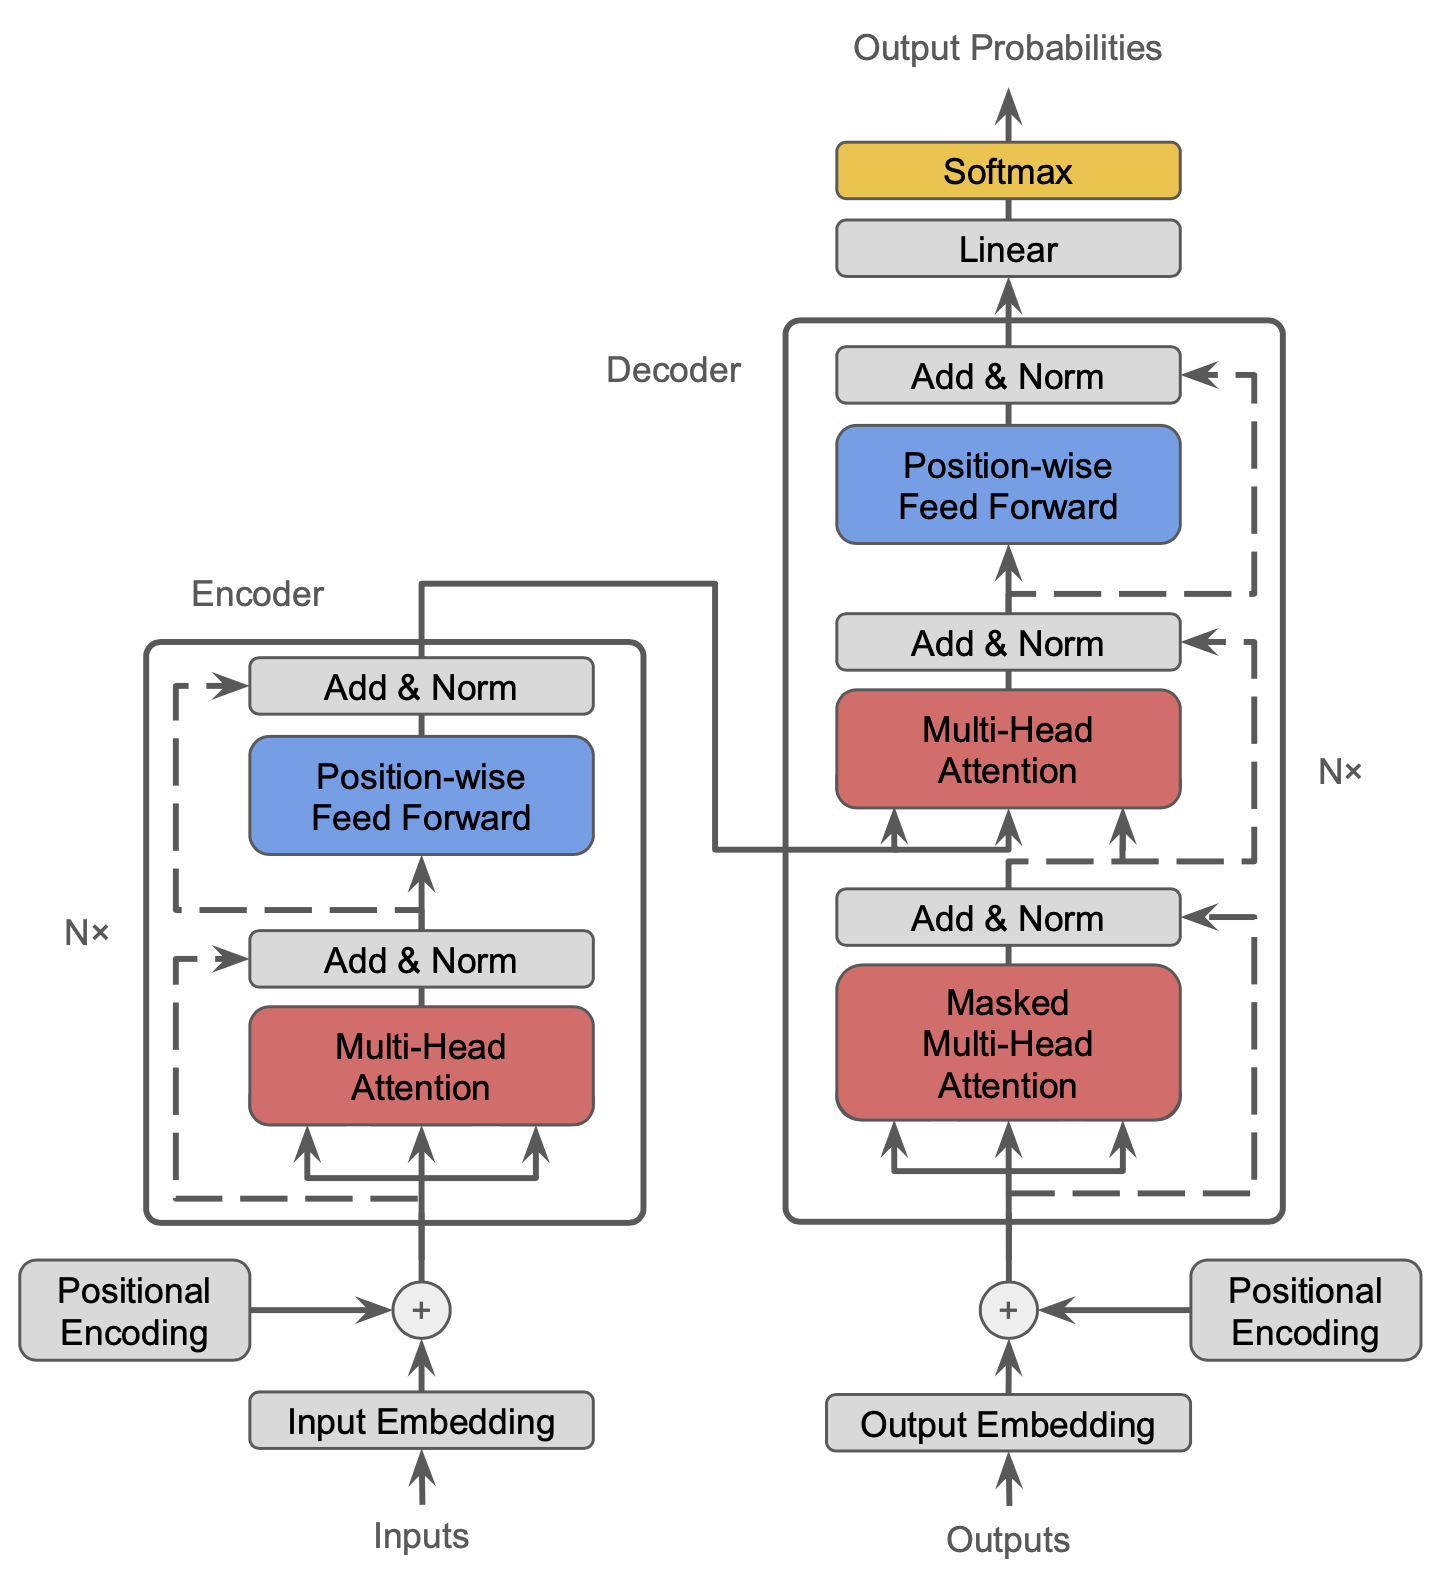
\includegraphics[width=\linewidth]{figures/transformer.png}
  \caption{The Transformer Model as described in \citet{vaswani2017attention}}
 \label{fig:transformer}
\end{figure}

An encoder block consists of a multi-head self-attention module followed by a position-wise fully-connected feed-forward network and contains additional add \& normalization steps. Decoder blocks are similar but contain a cross-attention layer inserted between the multi-head attention and feed-forward network layers.

The multi-head attention layers in \autoref{fig:transformer} can be broken down further, as shown in \autoref{fig:attentionlayer}, into $N$ linear and scaled dot-product attention layers corresponding to the $N$ number of heads. Following this, the outputs are concatenated and then projected via an additional linear layer. 

The scaled dot-product attention layer takes in three values as inputs: the query, key, and value matrices. Denoted as $Q$, $K$ (both of size $d_k$) and $V$ (of size $d_v$) respectively, these matrices are linearly projected $N$ times such that the query and key matrices are $N\times d_k$ and the value matrix is $N\times d_v$.
\begin{figure}[ht]
  \centering
  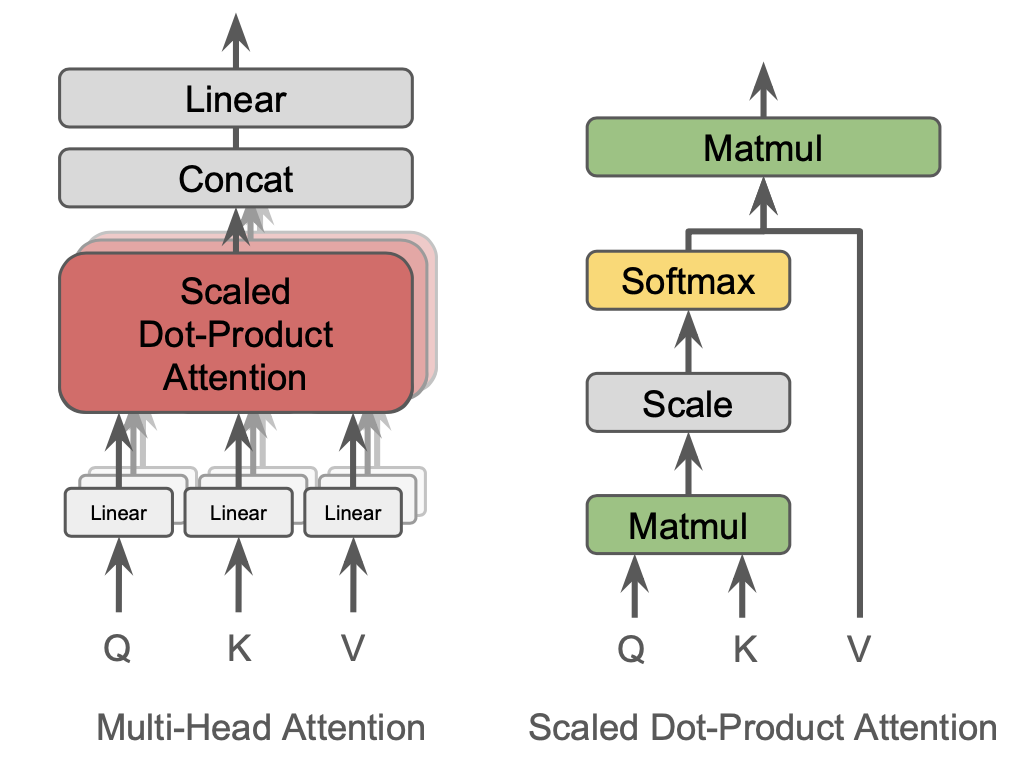
\includegraphics[width=\linewidth]{figures/attention.png}
  \caption{The Multi-Head Attention and Scaled Dot-Product Attention Layers}
 \label{fig:attentionlayer}
\end{figure}

First, the dot product of the query and key matrices is scaled by $\sqrt{d_k}$. The softmax is then applied to this matrix in order to get the weights of the values. Then, these weights are multiplied with the values matrix to get the final result. An illustration of the two matrix multiplication calculations is shown in \autoref{fig:qkvmats}.

\begin{figure}[t]
  \centering
  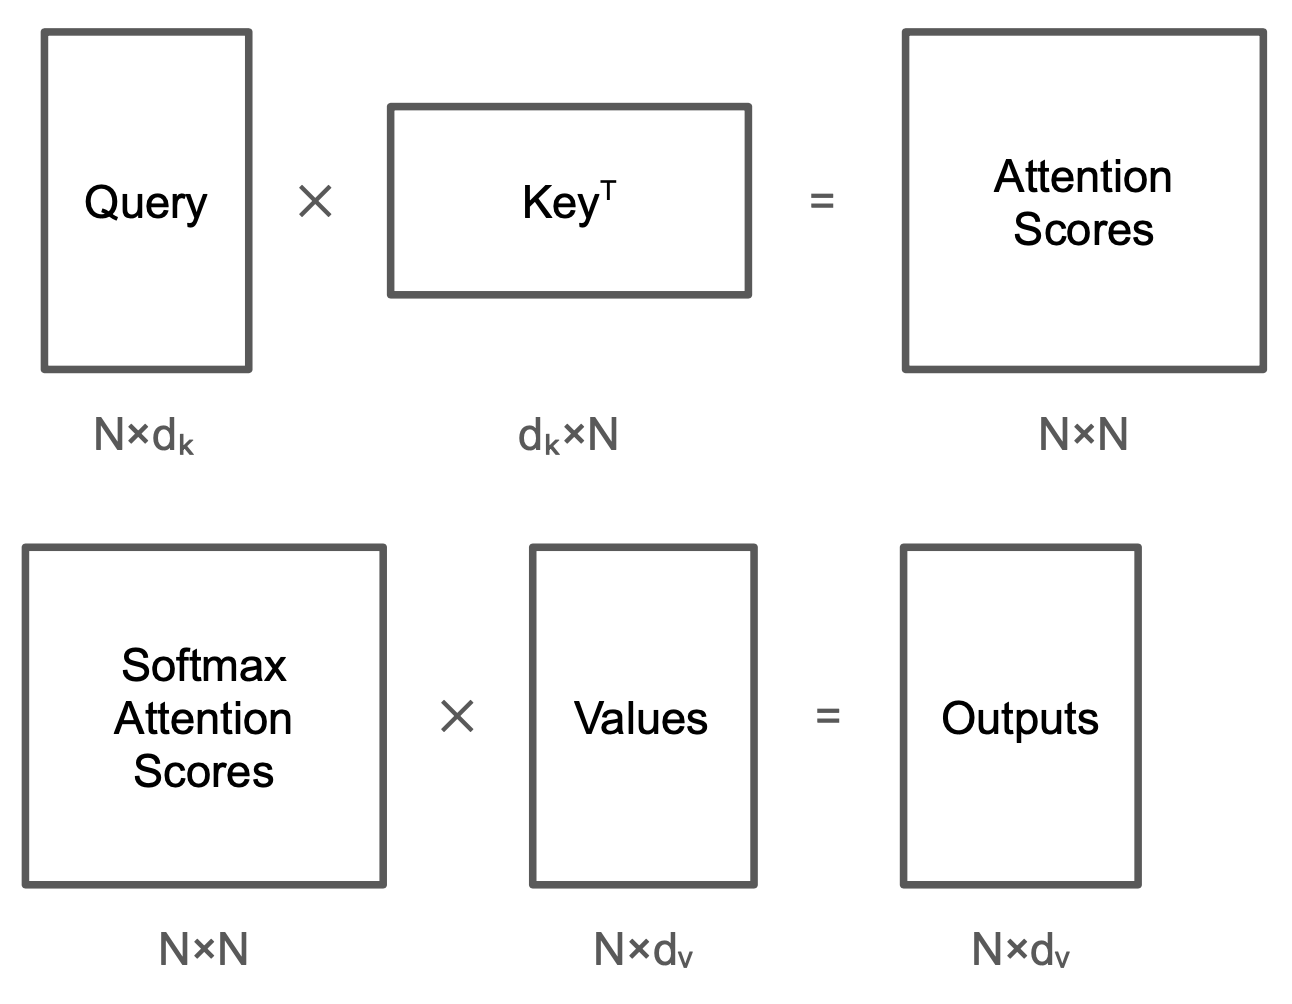
\includegraphics[width=\linewidth]{figures/qkvattn.png}
  \caption{Matrix Multiplication operations for the Scaled Dot-Product Attention Layers}
 \label{fig:qkvmats}
\end{figure}
\subsection{Attention}
The attention layer in particular plays a vital role in the Transformer as it allows the model to capture long-range relationships via similarity scores for all item pairs in a sequence \cite{khan2022transformers}.

Note that the complexity of self-attention is $O(T^2D)$, where $T$ is the sequence length and $D$ is the representation dimension. To validate this, we captured the computation time of layers within BERT\footnote{We used Hugging Face's BERT model \url{https://huggingface.co/docs/transformers/model_doc/bert}}, an encoder-only language model developed in 2018 \cite{devlin2018bert}. \autoref{fig:berttiming} shows that as the sequence length increases, the computational time of the self-attention layer, in dark red, scales quadratically. Also, it can be seen that self attention accounts for a large proportion of the entire computation time of a layer. Thus, optimizing attention is crucial to gaining speedup of computing a single transformer layer. The time, measured in seconds, is also shown in \autoref{fig:bertTimes} in the Appendix.
\begin{figure}[ht]
\pgfplotstableread{
    Label SelfAttention SelfOutput FeedForward Output topper
    128 0.079665  0.019992 0.084192 0.073205 0.001
    256 0.300243  0.040303 0.153612 0.147656 0.001
    512 0.545014 0.078534 0.322093 0.282523 0.001
    1024 3.854414 0.193473 0.686376 0.707752 0.001
    %2048 13.631169 0.332429 1.277496 1.172507 0.001
        }\testdata
    \centering
    \includegraphics[width=\linewidth]{bertTimingPlot.tikz}
    \caption{Computational Times for BERT layers vs Sequence Length}
    \label{fig:berttiming}
\end{figure}

\begin{figure*}[t]
  \centering
  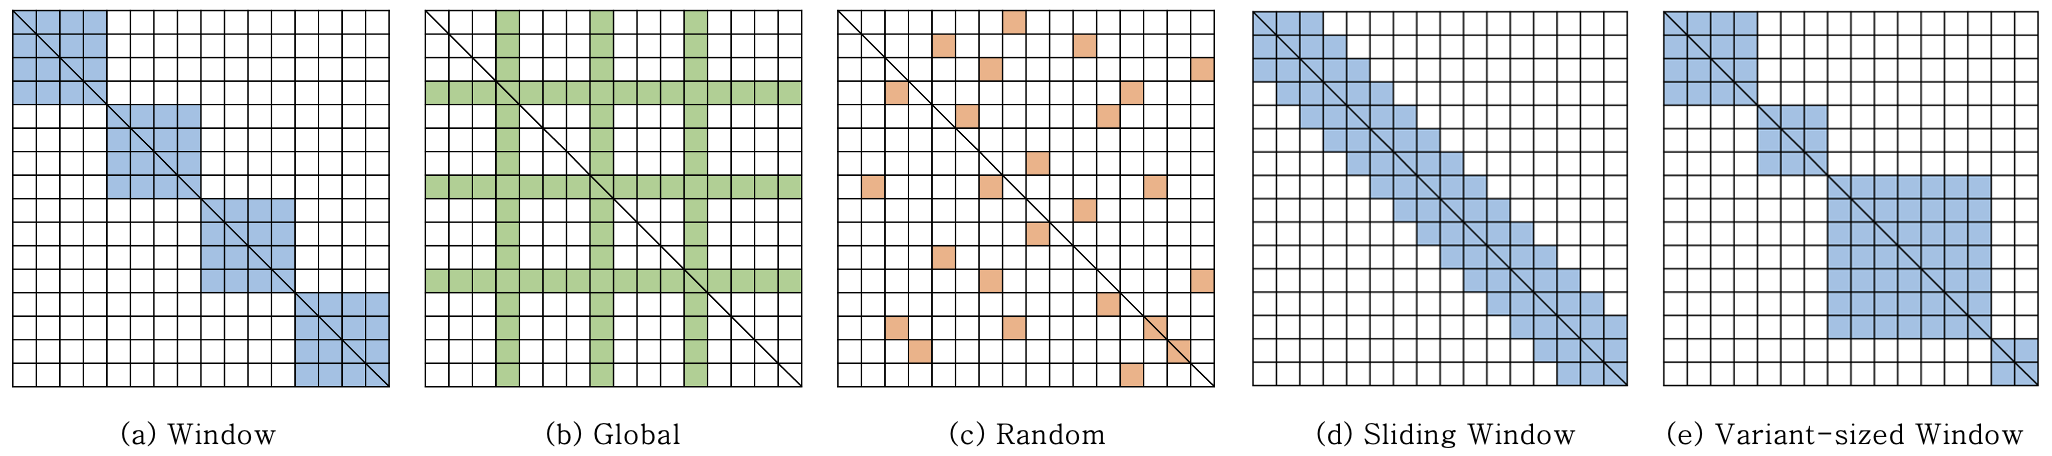
\includegraphics[width=\linewidth]{figures/building_block.png}
  \caption{Different factorization methods of sparse attention.  Each connectivity matrix shows whether an $i^{th}$ token (row) of a sequence refers to a $j^{th}$ token (column) to compute an attention score.}
 \label{fig:bulding_block}
\end{figure*}

Since both the memory and computational complexity scale quadratically with sequence length, attention becomes a performance bottleneck on longer sequences. One way to reduce computational costs is to introduce a sparsity bias into the attention module \cite{child2019generating}.
\subsection{Sparse Attention} \label{sub:sparse}
Sparse attention differs from normal attention in that it computes only a limited number of similarity scores for a sequence. By factorizing the attention matrix to only compute certain parts, sparse attention reduces the total computation complexity to $O(T\sqrt{T})$. Different factorization methods of the attention matrix lead to different sparse attention modes. Some such sparse attention modes are:


\begin{itemize}
    \item \textbf{Window attention}: Also known as \textit{block local attention}, window attention partitions the input sequence into equally sized blocks of some window size $ws$. All tokens in one block only attend to other tokens belonging to the same block. The resulting sparse attention scores matrix can be seen in \autoref{fig:bulding_block} (a). 
    
    \autoref{fig:bulding_block} (d) and (e) show variations on this mode. Sliding window or \textit{band attention}, uses a sliding window to ensure that tokens attend to neighboring tokens in the input sequence. Variant-sized Window partitions the input sequence into blocks of non-equal size. 
    \item \textbf{Global attention}: As shown in \autoref{fig:bulding_block} (b), global attention assigns particular tokens to calculate attention scores for all tokens in the sequence. The whole sequence then also attends to these selected tokens as well.
    \item \textbf{Random attention}: In \autoref{fig:bulding_block} (c), random attention samples edges randomly between tokens and computes their corresponding attention scores.  
\end{itemize}
\paragraph{Compound Sparse Attention}
Sparse attention models often combine multiple sparse attention modes to approximate full attention. For example, Longformer \cite{beltagy2020longformer}, as seen in \autoref{fig:longbird}, is a transformer-based model that uses a combination of sliding window and global attention. Meanwhile BigBird \cite{zaheer2020big} is an encoder-based pre-trained model that uses sliding window, global, and random attention.
\begin{figure}[t]
  \centering
  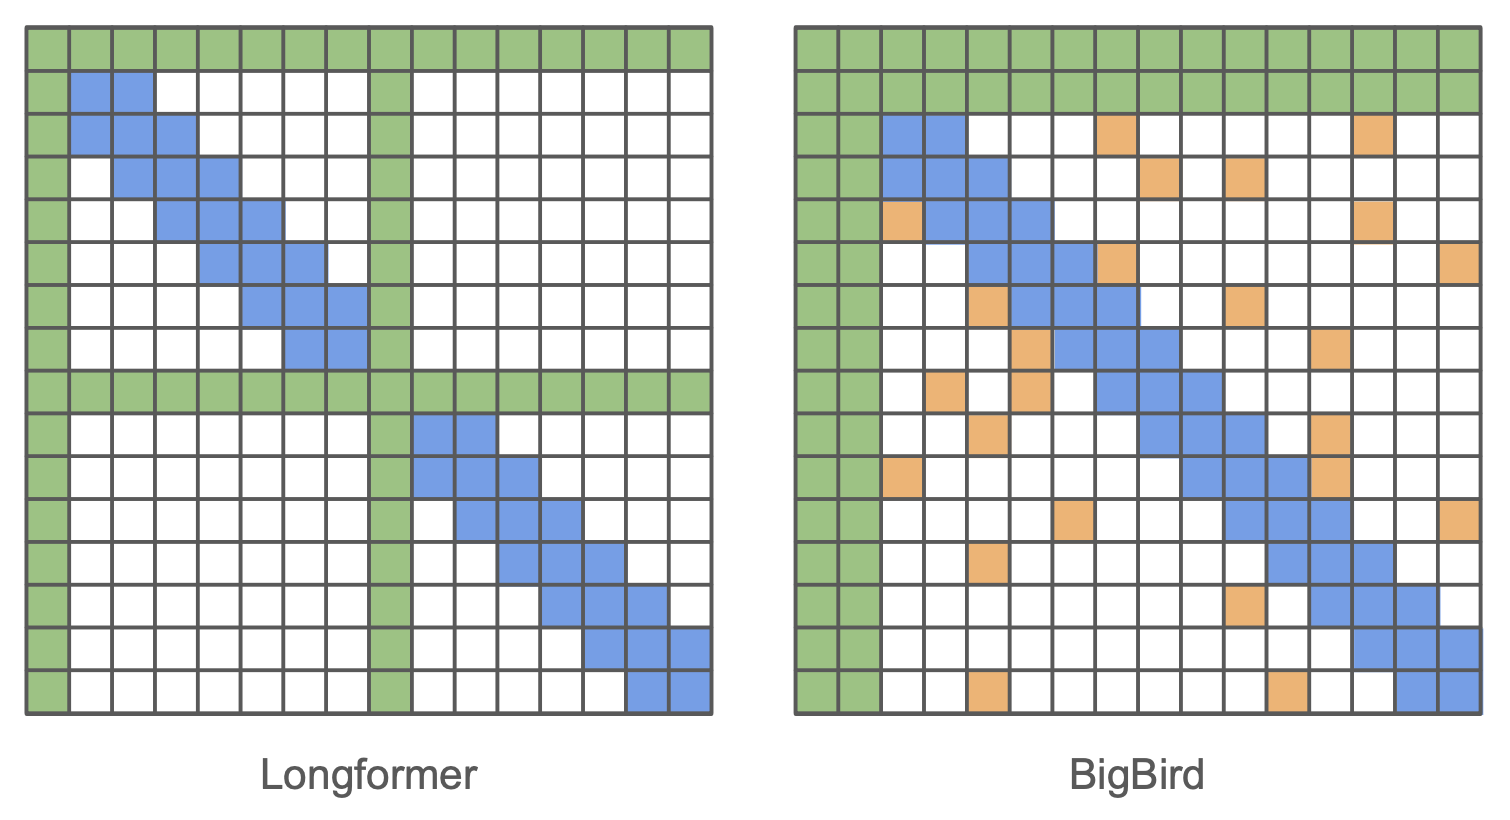
\includegraphics[width=\linewidth]{figures/longbird.png}
  \caption{Compound Sparse Attention factorization methods used in \citet{beltagy2020longformer} and \citet{zaheer2020big}.}
 \label{fig:longbird}
\end{figure}

\section{Approach}
In this section, we discuss general implementation details and the naive attention implementation. We then explain how we improved the performance of naive attention on GPU compared to CPU by optimizing GEMM (GEneral Matrix Multiplication).

\subsection{Technology}
We implemented three different sparse attention mechanisms---window, random, and global---on GPU using CUDA. For comparision, we also implemented a naive attention version on both CPU in C++ and GPU using CUDA. 

\subsection{Naive Attention Implementation}
We first discuss the naive multi-head full attention implementation on CPU. Then we will explain the motivations for parallelization.
\paragraph{Initializations} We first initialize the query, key, and value ($Q,K,V$) matrices to be N\_HEAD$\times N\times D$ ($D = d_k = d_v$), where N\_HEAD $=8$, $N=1024$, and $D = 64$. We define $AS$ to be the Attention Scores $N\times N$ matrix and $R$ to be the resulting $N\times D$ output matrix.

\begin{algorithm}
\caption{Scaled Dot Product Attention}
\begin{algorithmic}[1]
\Procedure{FullAttention}{$Q, K, V$} $\rightarrow R$
\EndProcedure
\State \Comment{Query $\times$ Key$^T$}
\ForAll{$d \in$ N\_HEAD; $i,j \in N$}
    \State $score \gets 0$
    \For{$d \in D$}
        \State $score \gets score + Q_{[h,i,d]} * K_{[h,j,d]}$
    \EndFor
    \State $AS_{[h,i,j]} \gets \frac{score}{\sqrt{d}}$
\EndFor
\State \Comment{Softmax}
\ForAll{$d \in$ N\_HEAD; $i \in N$}
    \State $sum \gets \sum AS_{[h,i,:]}$
    \State $AS_{[h,i,:]} \gets \frac{AS_{[h,i,:]}}{sum}$
\EndFor
\State \Comment{AS $\times$ Value}
\ForAll{$d \in$ N\_HEAD; $i \in N$}
    \State $sum \gets 0$
    \For{$d \in D$}
        \State $sum \gets sum + AS_{[h,i,:]} * V_{[h,:,d]}$
    \EndFor
    \State $R_{[h,i,d]} \gets sum$
\EndFor
\end{algorithmic}
\label{algorithm:scaled-dot-product}
\end{algorithm}

\paragraph{Pseudocode} As shown in \autoref{fig:attentionlayer} and \autoref{fig:qkvmats}, calculating attention involves two matrix multiplications, a softmax, and a scale. Algorithm \autoref{algorithm:scaled-dot-product} is a pseudocode for calculating attention. Lines 2 to 7 highlight the first matrix multiplication operation for the Query and Key matrices over all heads. Note that we combine the first matrix multiplication and scale step on Line 7 by dividing by $\sqrt{d}$ before assigning $score$ to the $AS$ matrix. Lines 8 through 11 are devoted to calculating the softmax over the attention scores matrix. Finally, Lines 12 to 17 detail the last matrix multiplication over all heads to calculate $R$.

\paragraph{Motivation for and Challenges of Parallelism}
As shown in our pseudocode, the Attention layer involves many matrix multiplication operations. These matrix multiplication operations can be highly parallelizable, since indices are not dependent on the output of other indices to calculate the dot product between a row and a column. However, when CUDA and \textit{sparse} attention are introduced to this situation, parallelizing becomes non-trivial since we have to optimize for both shared memory and various block/thread configurations depending on the sparse attention mode. Details on the exact block/thread configurations are discussed in \autoref{sec:sparse}.

Shared memory can reduce the number of global memory accesses in a program, thus speeding up performance. However shared memory is only useful when multiple threads are utilizing the same data. Luckily this is the case for matrix multiplication, as indices in a result matrix belonging to the same row (or column) both require the same entire row (or column) of the input matrices to calculate the dot product. Optimizations for shared memory using tiling methods are discussed in further detail in \autoref{sub:gemm}.

The introduction of the sparse attention calculation is particularly interesting. Now, we have to account for both Dense-Dense-Sparse (DDS) matrix multiplication in the first step of attention and Sparse-Dense-Dense (SDD) matrix multiplication in the last step of attention. Ultimately, this means that in our implementation each sparse attention mode required three separate kernels---a DDS matmul kernel, a softmax kernel, and a SDD matmul kernel---each with their own block/thread dimensions. Note that this also highlights an inherent dependency in attention: each kernel is dependent on the output of the last kernel.

\subsection{Optimizing GEMM} \label{sub:gemm}
cuBLAS \cite{cuBLAS} is a library by Nvidia that provides GPU-accelerated implementations of basic linear algebra subroutines. 
Specifically, for matrix multiplication, they use cache blocking to exploit shared memory efficiently.
We implemented cache blocking inside our CUDA kernels based on this approach.

\begin{figure}[t]
  \centering
  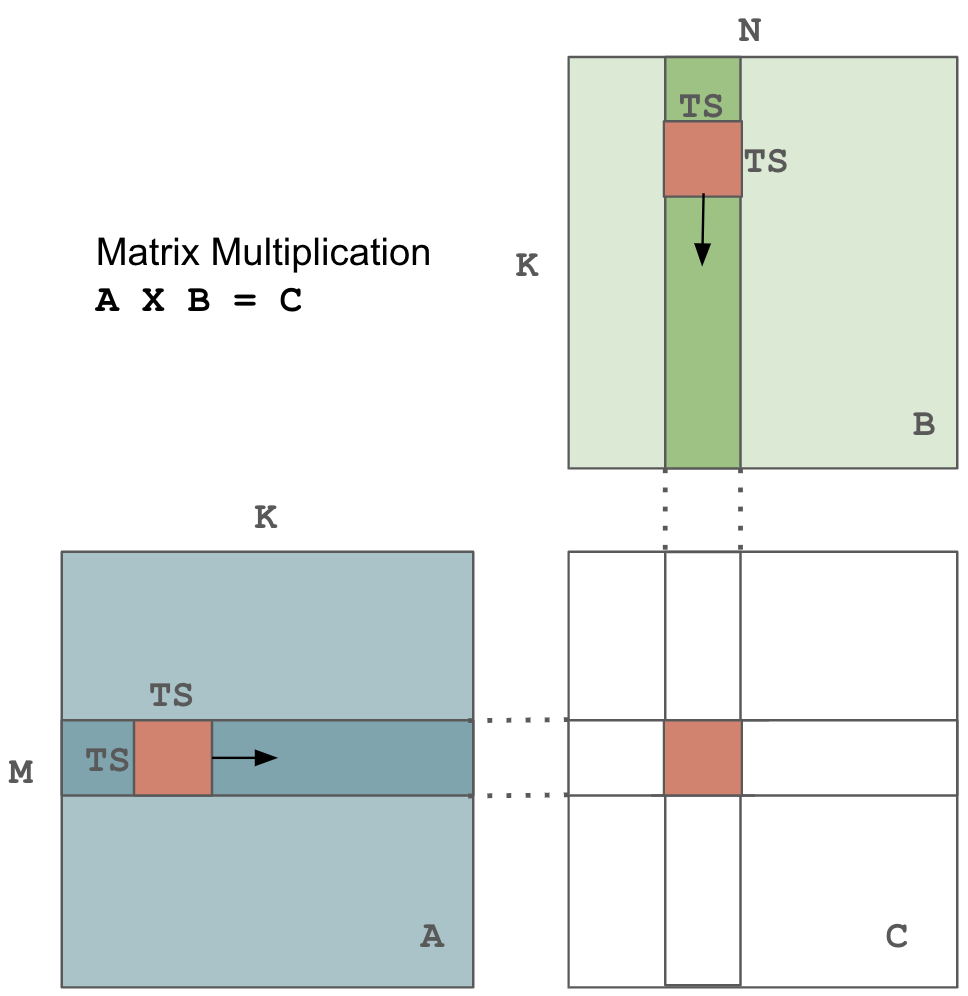
\includegraphics[width=\linewidth]{figures/cache_block_gemm.png}
  \caption{GEMM (GEneral Matrix Multiplication) using cache block on shared memory. Advance tiles of \texttt{TS} $\times$ \texttt{TS} cache block on shared memory to calculate red region of C.}
 \label{fig:cache_block_gemm}
\end{figure}

\autoref{fig:cache_block_gemm} illustrates how cache blocks are used in matrix multiplication operations. Instead of accessing matrices \texttt{A} and \texttt{B} in global memory, the threads belonging to the same block exploit shared memory. However since shared memory is limited, instead of loading entire rows and columns from \texttt{A} and \texttt{B} respectively, we define a \texttt{TS} $\times$ \texttt{TS} (\texttt{TS} standing for tile size) block that loads partial blocks of rows from \texttt{A} and columns from \texttt{B} onto shared memory. The number of threads per block is defined as \texttt{(H, TS, TS)}, where \texttt{H} is the number of heads in multi head attention.

\begin{figure*}[t]
  \centering
  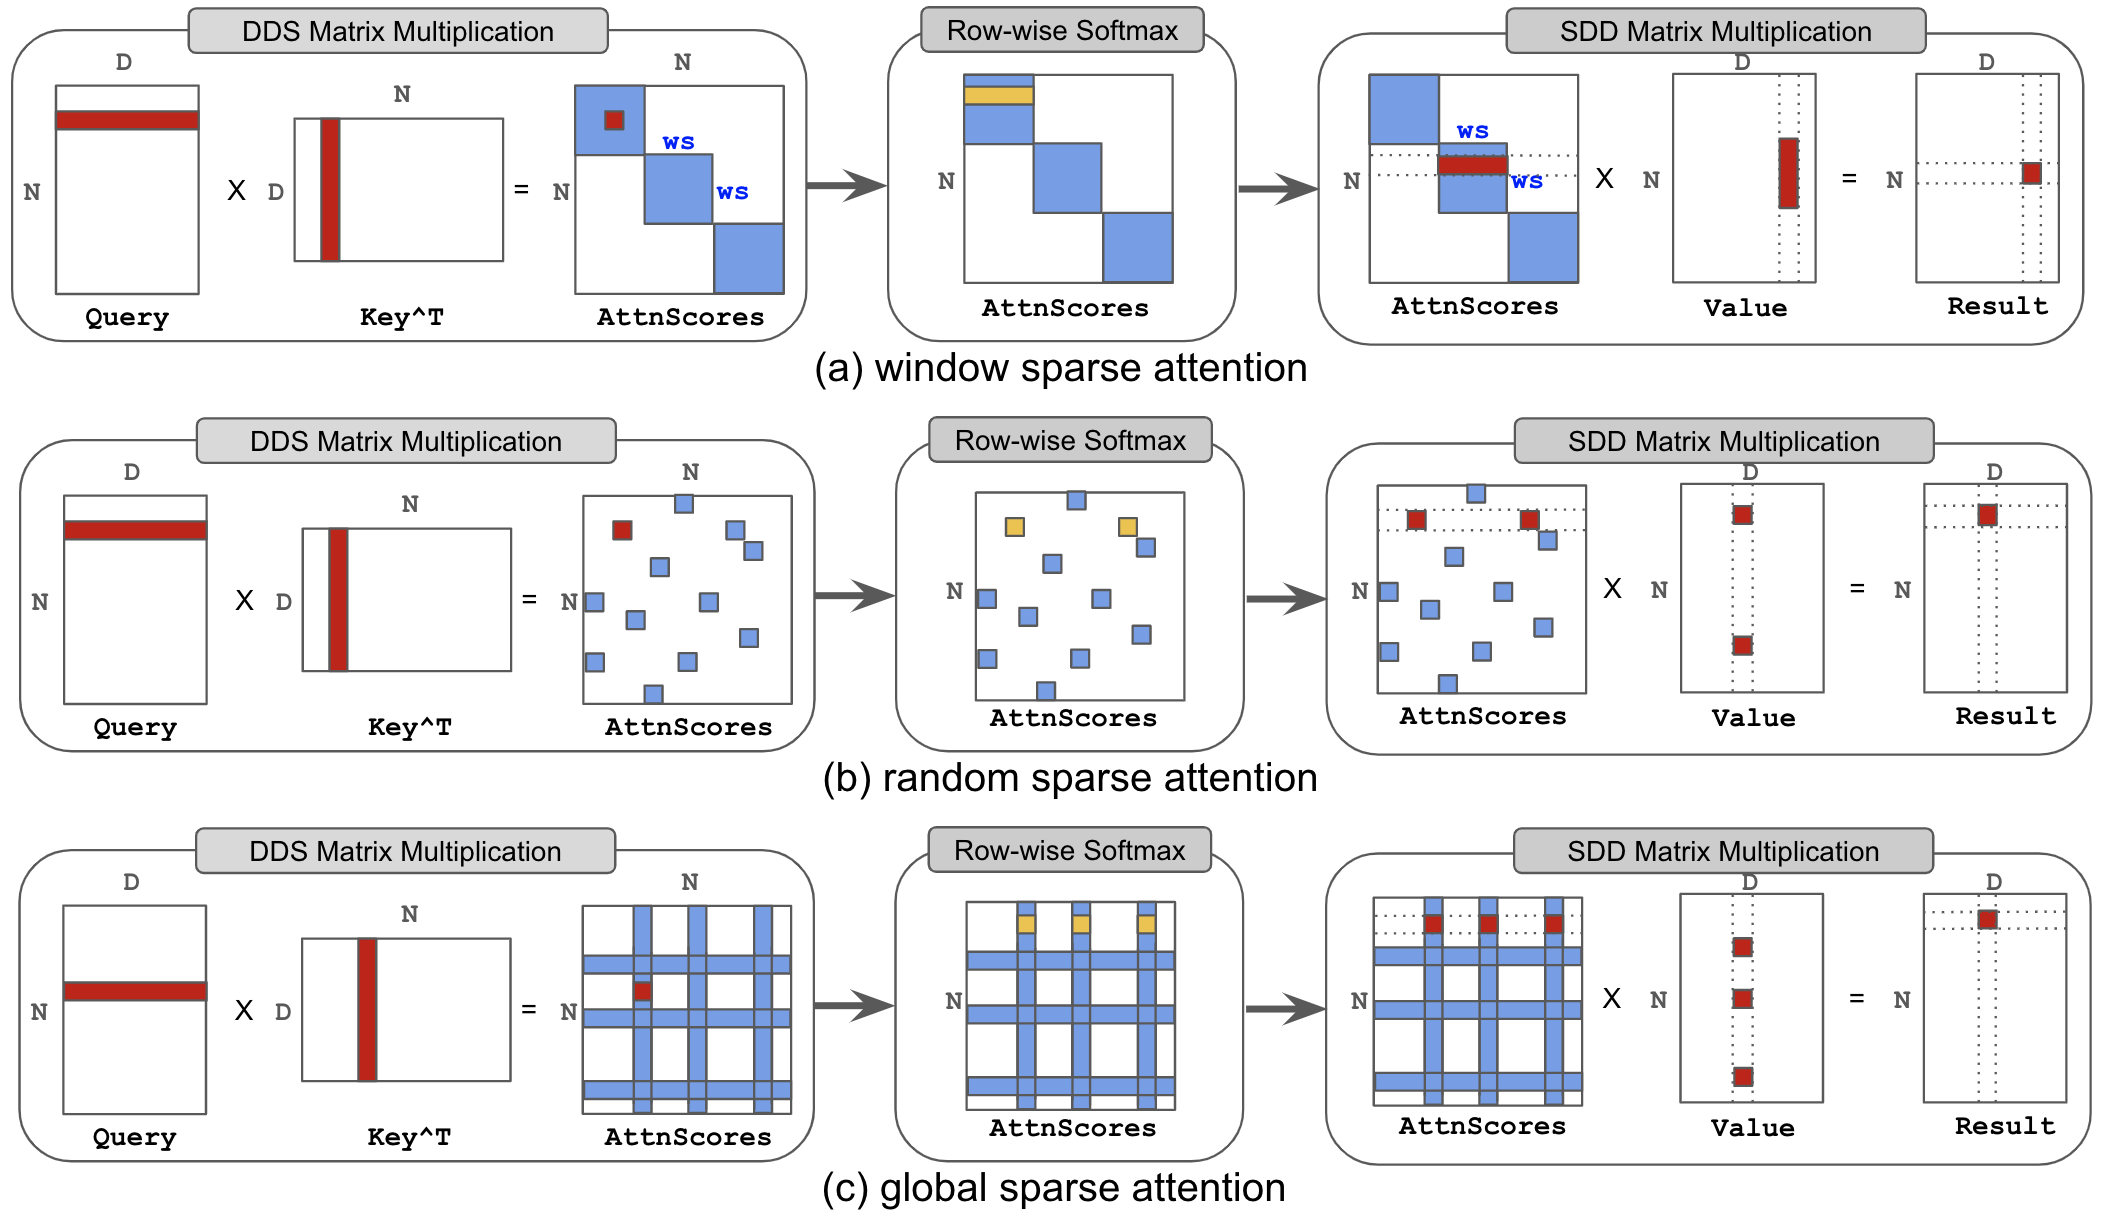
\includegraphics[width=\linewidth]{figures/sparse_attn.png}
  \caption{Three modes of sparse attention. DDS (Dense-Dense-Sparse) matrix multiplication kernel is used for \texttt{Query} $\times$ \texttt{Key} to produce the sparse attention score matrix. Softmax is done row-wise on valid attention scores. SDD(Sparse-Dense-Dense) matrix multiplication is used for \texttt{AttnScores} $\times$ \texttt{Value} for the final output. Blue parts in \texttt{AttnScores} show valid attention scores. Red shows an example of calculating an element in the resulting matrix. Yellow gives an example of the elements that are considered for row-wise softmax for a single row. \texttt{N} is sequence length, and \texttt{D} is model dimension.}
 \label{fig:sparse_attn}
\end{figure*}

Thus, as we perform matrix multiplication for some group of rows and columns in \texttt{A} and \texttt{B}, we compute a smaller subset of this larger calculation using the block and accumulate the result as the block is advanced along the row or column. The final result is then the summation of the smaller tile matrix multiplications. 

This method substantially improves performance because the rows and columns are reused by different threads. As a toy example, assume we perform matrix multiplication with a tile size \texttt{TS=4}. Referring to \autoref{fig:cache_block_gemm}, in order to calculate \texttt{C[1][2]} we need to compute the dot product of row 1 in \texttt{A} and column 2 in \texttt{B}. Note that another thread assigned to calculate \texttt{C[1][3]} will need row 1 in \texttt{A} and column 3 in \texttt{B}. And more generally, all threads neighboring the \texttt{C[1][2]} calculation will need to access similar rows and columns of \texttt{A} and \texttt{B}. Thus, splitting rows and columns into blocks that can fit on shared memory will reduce redundant accesses to global memory. 

\subsection{Other Approaches}
Prior to researching this particular optimization strategy, we naively implemented the CUDA kernel by parallelizing the threads across different heads.
We expected that this implementation would not generate significant speedup gains, but might be faster than the CPU version due to the fact that perhaps some of the work would be parallelized.

Contrary to our expectations, using the naive approach on the the window sparse CUDA kernel was 4.17x \textit{slower} than the same window sparse code implemented for CPU. 
From this we realized that using CUDA kernels in an inefficient way slows down the task even compared to the CPU.

\section{Sparse Attention}\label{sec:sparse}
We implemented multi-head attention for a single layer of the transformer. We designed three different CUDA kernels for each sparse attention mode: \texttt{MultiHeadDDS}, \texttt{MultiHeadSoftMaxSparse}, and \texttt{MultiHeadSDD}. Instead of doing a general matrix multiplication operation or full softmax, each kernel takes in a user-defined configuration as an argument, and performs sparse matrix multiplication or sparse softmax based on that configuration.

In the following subsections, we explain how we implemented each sparse attention mode in detail.



\subsection{Window Attention}
\autoref{fig:sparse_attn} (a) shows how window sparse attention is calculated. Given a user-configurable parameter \texttt{ws}, the goal of \texttt{MultiHeadDDS} kernel is to calculate an attention score connectivity matrix \texttt{AttnScores}. The \texttt{AttnScores} matrix for window sparse attention calculates attention scores for regions of size \texttt{ws} $\times$ \texttt{ws} along the diagonal. Intuitively, this means that a token will only \textit{pay attention} to nearby tokens. We only calculate the attention scores for the pre-configured regions and do not perform any checks for whether a element is within the region or not inside the kernel. This also improves the performance of the kernel.

For window sparse attention, \texttt{MultiHeadDDS} kernel combines block cache optimization with windows. Each \texttt{ws} $\times$ \texttt{ws} within \texttt{AttnScores} is split up into \texttt{TS} $\times$ \texttt{TS} regions, so that the threads within the same block can access the same rows or columns needed on shared memory.

After calculating the sparse \texttt{AttnScores} matrix, we launch \texttt{MultiHeadSoftMaxSparse} kernel with configurations. This kernel performs row-wise softmax for valid attention scores in the \texttt{AttnScores} matrix. The threads also exploit shared memory after loading and accessing a row on shared memory to sum the total for the row, rather than accessing global memory to sum the total.

Finally, the \texttt{AttnScores} matrix is passed onto the \texttt{MultiHeadSDD} kernel for sparse matrix multiplication with the \texttt{Value} matrix. We launch a thread for every element in the resulting dense matrix. Each thread exploits shared memory of \texttt{TS} $\times$ \texttt{TS} by loading sub parts of rows of \texttt{AttnScores} and sub parts of columns of \texttt{Value} on shared memory.

\subsection{Random Attention}
\label{sec:random-attn}
The process of calculating random sparse attention is illustrated in \autoref{fig:sparse_attn} (b). The overall implementation is similar to window sparse attention. However, the valid target attention scores in the \texttt{AttnScores} are randomly chosen. Intuitively, this means that some token will \textit{pay attention} to other random tokens. 

Due to this randomness, it is impossible to exploit shared memory. Specifically, for \texttt{MultiHeadDDS}, we launch threads for every valid element in the \texttt{AttnScores} matrix as we did for window sparse. However, since nearby threads do not always make accesses to the same row or column of the \texttt{Query} or \texttt{Key} matrix, there is no point of exploiting shared memory.

For fair comparison with window sparse attention, we define a user-configurable parameter \texttt{RF}, or Random Fraction, which controls the proportion of elements per row (with respect to the sequence length \texttt{N}) to choose as target elements in the \texttt{AttnScores} matrix. However, due to the fact that we cannot exploit shared memory, choosing an \texttt{RF} to match the amount of computation performed in window sparse results in a much longer execution time. The details of this are discussed in \autoref{sec:main-result}.

\subsection{Global Attention}
Calculations for global sparse attention are shown in \autoref{fig:sparse_attn} (c). Global attention varies slightly from random and window sparse attention in that global tokens are selected along the diagonal of the sparse matrix. Notice that if all the tokens along the diagonal are selected to be global, then global sparse attention will mimic the behavior of full attention (since all tokens will attend to all tokens). 

Some token configurations make it easier to utilize shared memory than others. Take, for instance, the grid pattern shown in \autoref{fig:sparse_attn} (c) as compared to the grid pattern shown in \autoref{fig:longbird} of the Longformer and BigBird models. Notice how in both Longformer and BigBird, the first k tokens along the diagonal are chosen to be global tokens (contiguous tokens), while in \autoref{fig:sparse_attn} (c), the global tokens are more spread out over the diagonal (grid-like tokens). 

Picking global tokens to cover contiguous regions of the sparse matrix simplify attention score calculations, since the total sparse area can be decomposed into two blocks: a horizontal block across the top of the sparse matrix, and a vertical block along the left side of the sparse matrix. Choosing contiguous tokens might also improve memory locality, since accessed rows and columns are all neighbors of each other.

Calculating the \texttt{AttnScores} for grid-like global tokens is done in two passes with two kernels. The first pass (the 'grid-like' kernel) calculates the attention scores of the columns of the sparse matrix while the second pass (the full row kernel) calculates the scores for the rows. While this results in redundant calculations at the grid vertices, it is also the simplest approach that maintained consistent block dimensions.

The \texttt{MultiHeadSoftMaxSparse} kernel is launched twice as well. The first launch handles the \texttt{AttnScores} rows whose diagonal indices are not global tokens, while the second launch handles the full rows whose are. Similar logic is applied when calculating the output matrix using \texttt{MultiHeadSDD}; one kernel handles non-full rows while the another handles full rows.

Both \texttt{MultiHeadSDD} and \texttt{MultiHeadDDS} implement the tiling method discussed in \autoref{sub:gemm}. For fair comparison with random and window sparse, we also define a user-configurable variable \texttt{ID}, which denotes the number of global tokens selected along the diagonal.

\renewcommand{\arraystretch}{1.2}
\setlength{\tabcolsep}{7.5pt}
\begin{table*}[t]
\small
\centering
% =====================================================================
%                           Naive Attn
% =====================================================================
\begin{subtable}{\textwidth}\centering
\begin{tabular}{||c|c|c||}
\hline
Sequence Length & CPU ver & GPU ver GEMM kernel \\ [0.5ex] 
\hline\hline

128 & 7387 & 90.11 \\
256 & 25711 & 291.65 \\
512 & 110313 & 1063.26 \\
1024 & 390943 & 8273.95 \\

\hline
\end{tabular}
\caption{Naive (full) attention on CPU and GPU}
\end{subtable}
% =====================================================================
%                           Window Attn
% =====================================================================
\begin{subtable}{\textwidth}\centering
\begin{tabular}{||c|ccc|c||}
\hline

Sequence Length & DDS & SoftMaxSparse & SDD & Total \\ [0.5ex] 

\hline\hline

128 & 15.55 & 10.24 & 10.62 & 36.41 \\
256 & 19.42 & 10.53 & 10.70 & 40.65 \\
512 & 22.21 & 10.24 & 10.72 & 43.17 \\
1024 & 36.86 & 13.12 & 14.34 & 64.32 \\

\hline
\end{tabular}
\caption{Window-sparse attention on GPU}
\end{subtable}
% =====================================================================
%                           Random Attn
% =====================================================================
\begin{subtable}{\textwidth}\centering
\begin{tabular}{||c|c c c|c||}
\hline
Sequence Length & DDS & SoftMaxSparse & SDD & Total \\ [0.5ex] 
\hline
\hline
128 & 6.25 & 6.02 & 14.33 & 26.61 \\
256 & 6.24 & 6.27 & 25.40 & 37.91 \\
512 & 6.27 & 6.14 & 71.45 & 83.87 \\
1024 & 6.75 & 6.88 & 248.19 & 261.82 \\

\hline
\end{tabular}
\caption{Random-sparse attention on GPU}
\end{subtable}
% =====================================================================
%                           Global Attn
% =====================================================================
\begin{subtable}{\textwidth}\centering
\begin{tabular}{||c|ccc|c||}
\hline
Sequence Length & DDS & SoftMaxSparse & SDD & Total \\ [0.5ex] 
\hline\hline

128 & 26.62 & 14.08 & 35.94 & 76.64 \\
256 & 30.72 & 14.34 & 49.86 & 94.91 \\
512 & 43.01 & 47.10 & 90.30 & 180.42 \\
1024 & 72.03 & 104.45 & 182.18 & 358.66 \\

\hline
\end{tabular}
\caption{Global-sparse attention on GPU}
\end{subtable}
% =====================================================================
% =====================================================================
\caption{Breakdown and total execution time of attention for the naive (full) attention on CPU and GPU, and three different sparse attention modes on GPU. All experiments used \texttt{num head = 8}, \texttt{D = 512}, and \texttt{TS = 8} (if applicable). All values are in microseconds.}
\label{table:main_exp}
\end{table*}

\section{Experiments}
\label{sec:main-result}
\subsection{Experimental setup}
We implemented naive full attention on CPU and sparse attention on GPU using CUDA. We treat the single-threaded CPU version as our benchmark.
\paragraph{Timing} To calculate the elapsed time for our CPU implementation, we used \texttt{std::chrono::steady-clock::now()}. For GPU timing, we used CUDA events. Specifically, we used \texttt{cudaEventCreate()}, \texttt{cudaEventRecord()}, \texttt{cudaEventSynchronize()} and \texttt{cudaEventElapsedTime()} to track the elapsed time. We also made sure that we used \texttt{cudaDeviceSynchronize()} for synchronization. 

\paragraph{Initialization} We generated random floating point query, key, and value matrices and used \texttt{cudaMemCpy} so that they can be on device memory.

Experiments were conducted on GHC machines, using a single NVIDIA GeForce RTX 2080 GPU.

\subsection{Main Result}
\autoref{table:main_exp} shows the results for our kernels.

Looking at \autoref{table:main_exp} (a), it can be seen that execution time increases quadratically to the sequence length for the naive full attention implementation. However, note that using a well-optimized general matrix multiplication kernel for attention on GPU can result in up to 103x speedup for some sequence lengths. 

\autoref{table:main_exp} (b) shows the results of window sparse attention on GPU using block cache optimization with window size \texttt{ws = 16}. Overall this version takes less time than the full GEMM on GPU and does not scale quadratically to the sequence length.

Random sparse attention results are illustrated in \autoref{table:main_exp} (c). We configured the \texttt{RF} hyperparameter for fair comparison of using \texttt{ws = 16} for window-sparse attention. Random sparse attention takes longer to execute compared to window and exhibits quadratic scaling, similar to the naive full attention. This is likely due to the fact that it does not exploit shared memory, which can severely impact performance on CUDA.

\autoref{table:main_exp} (d) shows the execution time of the global sparse attention implementation on GPU using grid-like global tokens and \texttt{ID = 16}. Overall, global sparse attention appears to take more time than both the window and random sparse attention methods. Notice that it also exhibits nonlinear scaling. This might be due to various reasons including ineffective shared memory utilization and also the fact that there are most calculations in general needed as sequence length increases. Part of this slow performance might also be due to the redundant calculations performed for the grid vertices, since both the grid-like kernel and the full kernel compute these entries.
\section{Ablation Studies}

\subsection{Kernel Breakdown Analysis}
In this section, we breakdown the runtime of the three kernels: \texttt{MultiHeadDDS}, \texttt{MultiHeadSoftMaxSparse}, and \texttt{MultiHeadSDD}. \autoref{table:main_exp} shows the runtimes of each kernel for the three sparse attention modes.

\paragraph{Window Sparse Attention} For window sparse attention, kernel \texttt{MultiHeadSoftMaxSparse} takes a similar amount of time for all sequence lengths. This is because the experiments were conducted using a fixed window size (\texttt{ws = 16}) and the task was well-parallelized across threads.

\texttt{MultiHeadSDD} also shows similar execution time for all sequence lengths. Since the kernel is launched with multiple blocks and threads, each thread is responsible for a single element in the \texttt{N} $\times$ \texttt{D} output matrix. Thus, it is not affected by the sequence length \texttt{N}. 

However, it can be seen that the \texttt{MultiHeadDDS} kernel scales with the sequence length. This is because a longer sequence length entails more computations overall, since there are more \texttt{ws} $\times$ \texttt{ws} blocks in the resulting \texttt{AttnScores} matrix.

\paragraph{Random Sparse Attention} For random sparse attention in \autoref{table:main_exp} (c), \texttt{MultiHeadDDS} exhibits similar times for all sequence lengths. This is because the experiment was designed to compute a similar number of elements in the output matrix for all sequence lengths. 


However, note that it takes less time than window sparse \texttt{MultiHeadDDS}. We believe this might be because very few elements are calculated for the \texttt{AttnScores} matrix and in that case using shared memory could add overhead (due to numerous calls to \texttt{syncthreads()}).

We also noticed that \texttt{MultiHeadSDD} is the main bottleneck for random attention. 
We claim this is due to two reasons:
\begin{enumerate}
    \item The random sparse kernel does not exploit shared memory since nearby threads usually don't access the same rows or columns
    \item Unlike window sparse's \texttt{MultiHeadSDD}, which accesses contiguous regions in memory (see \autoref{fig:sparse_attn} (a)), random sparse's kernel accesses random elements \textit{in the same column} of the \texttt{Value} matrix, which is an inefficient access pattern for row-major-ordered matrices.
\end{enumerate}
\paragraph{Global Sparse Attention}
For global sparse attention, all three kernels appear to scale nonlinearly. As mentioned before this might be due to poor shared memory utilization, since our implementation of global sparse attention accesses noncontiguous vertical columns for each kernel pass, which is inefficient since our matrices use row-major-order. 

This bottleneck can also be seen in \autoref{fig:globalZoom}, which shows the execution times of the grid-like kernels compared to the full row kernels. Notice that while DDS and SSD seem to take the same amount of time regardless of which kernel pass is being launched, softmax has a significant execution time difference between grid-like and full. Most notably, the softmax kernel responsible for the non-full rows of the attention matrix performs extremely slowly, highlighting that when shared memory is used to access noncontiguous columns, performance suffers.

However, one interesting thing to note in \autoref{table:main_exp} is that for random sparse's \texttt{MultiHeadSDD}, global sparse's \texttt{MultiHeadSDD} had a faster execution time. This might be because global sparse utilizes shared memory more effectively than random sparse in that circumstance. 

\begin{table}[t]
\small
\centering
\renewcommand{\arraystretch}{1.2}
\setlength{\tabcolsep}{7.5pt}
% =====================================================================
%                           Window sparse
% =====================================================================
\begin{subtable}{\linewidth}\centering
\begin{tabular}{||c|c||}
\hline

\texttt{ws} & Total \\ [0.5ex] 

\hline\hline

16 & 58.11 \\
32 & 97.60 \\
64 & 184.32 \\


\hline
\end{tabular}
\caption{Window-sparse attention on GPU ablation. \texttt{ws} is window size.}
\end{subtable}
% =====================================================================
%                           Random sparse
% =====================================================================
\begin{subtable}{\linewidth}\centering
\begin{tabular}{||c|c||}
\hline

\texttt{RF} & Total \\ [0.5ex] 

\hline\hline

0.02 & 258.40 \\
0.1 & 1337.98 \\
0.2 & 2708.16 \\
0.4 & 5350.53 \\
0.6 & 8139.29 \\


\hline
\end{tabular}
\caption{Random-sparse attention on GPU ablation. \texttt{RF} is the random fraction.}
\end{subtable}
% =====================================================================
%                           Global sparse
% =====================================================================
\begin{subtable}{\linewidth}\centering
\begin{tabular}{||c|c||}
\hline

ID & Total \\

\hline\hline
16 & 344.06 \\
32 & 518.14 \\
64 & 685.66 \\


\hline
\end{tabular}
\caption{Global-sparse attention on GPU ablation. \texttt{ID} is the number of global indices.}
\end{subtable}
\caption{Ablations. Total is the total execution time for all kernels (DDS, softmax, SDD). Experiments are done on sequence length \texttt{N = 1024}.}
\label{table:ablation}
\end{table}
\begin{figure}[ht]
\pgfplotstableread{
    Label Grid-like Full topper
    DDS   44.44  34.82 0.001
    SM   105.82  5.63 0.001
    SDD  83.97  109.76 0.001
        }\testdata
    \centering
    \includegraphics[width=\linewidth]{globalPlot.tikz}
    \caption{Global-sparse attention on GPU. Experiments are done on sequence length \texttt{N = 1024}, and with \texttt{ID = 16} global tokens. First pass (i.e. DDS$_1$, SM$_1$, SDD$_1$) target grid-like rows while the second pass targets full rows. Table of values can be found in \autoref{sec:appendix}.}
    \label{fig:globalZoom}
\end{figure}

\subsection{Changing Hyperparameters}
To see how changing user configurations (i.e. hyperparameters) affects sparse attention, we conducted experiments for different hyperparameter values for each of the sparse attention modes. \autoref{table:ablation} (a) shows the total execution time on varying window sizes. As expected, the total execution time scales linearly ($O(N)$) to the window size.

Random sparse attention in \autoref{table:ablation} (b) shows interesting results. As expected, the total execution time increases as the random fraction increases. However for \texttt{RF = 0.6}, the execution time is similar to that of the naive full attention version on GPU with the same sequence length 1024 (\autoref{table:main_exp} (a)). This is surprising since \texttt{RF = 0.6} calculates attention scores for only 60\% of the full attention scores matrix, while the naive full attention on GPU calculates the attention score for all elements. From this we can see that inefficient usage of shared memory can greatly impact kernel performance.

In \autoref{table:ablation}, global sparse attention exhibits increasingly slower execution times as \texttt{ID} increases. This is partially expected because \texttt{ID} is directly correlated with the number of full-row attention calculations required for our attention scores matrix. However, as mentioned before in the previous section, this performance may also be attributed to shared memory inefficiencies.

\section{Limitations and Conclusion}
One limitation that applies to all of our sparse attention implementations is that we use three different kernels, resulting in three different CUDA kernel launches. Since each kernel launch adds additional time, we believe that fusing the three kernels into a single attention kernel could have helped improve performance. However, this was difficult to achieve and was not implemented since work assignment to threads varied by layer (i.e. DDS multiplication, softmax, SDD multiplication).

Additionally random sparse attention's inherently random accesses hinders its usage of share memory, which greatly limited performance. Despite this, we believe it is possible to analyze the randomly generated indices and come up with an optimal way of exploiting shared memory. However, coming up with this algorithm is nontrivial and not feasible given our timeline. Note that this also applies to the methods used for global sparse attention.

Also, a multi-threaded CPU implementation for comparison with SIMD on GPU could have provided interesting comparisons between SIMD instructions on CPU and GPU. However, given our original timeline for this project, this was also not implemented.

Additionally, our method currently only measures the performance and not the accuracy of a single multi-head attention layer. In reality, to test whether our CUDA implementations are able to approximate full attention accurately, we would have to build out the entire model end-to-end, which was not in the scope of this project.

As mentioned in \autoref{sub:sparse}, sparse attention models are usually comprised of multiple sparse attention modes, and not just window, random, or global as shown in our work. Measuring the performance of multiple combinations of these modes in CUDA is also a potential extension of our work.

Sparse matrices are memory inefficient since many of the indices held in memory are never utilized. Our method maintained a large focus on DDS and SDD matrix multiplication and thus did not target memory efficiency. Memory efficient matrix multiplication algorithms that utilize matrix representations, such as the Block Compressed Sparse Row (BCSR) \cite{giannoula2022sparsep}, Compressed Sparse Block format (CSB) \cite{bulucc2009parallel}, and ELLPACK \cite{bell2009implementing} storage formats might result in better utilization of memory. 

\begin{figure}[t]
  \centering
  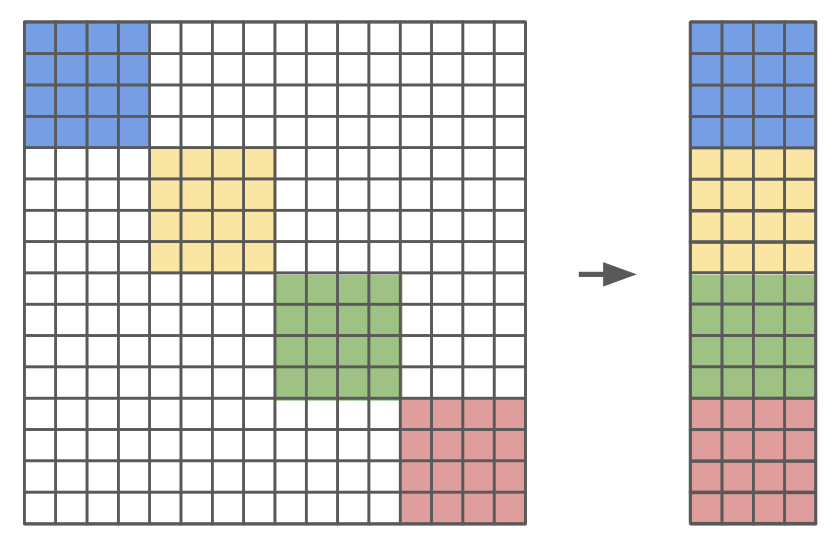
\includegraphics[width=\linewidth]{figures/dense.png}
  \caption{A possible dense representation of the window sparse attention matrix.}
 \label{fig:dense}
\end{figure}

Considering a blocked-ELLPACK \cite{blockedEll} format for window, the sparse matrix can be trivially compressed as the number of non-empty elements per row is equal throughout, as shown in \autoref{fig:dense}. However for global and random, their matrix compression could possibly be more involved. Random's row element indices are randomly sampled and their positions needed to be encoded into this compressed format. Since global contains uneven non-empty row elements, traditional ELLPACK which pads uneven rows with 0s might yield no memory storage difference. As such other compression methods could be further explored.

We hope that our investigation into the performance of these sparse attention modes, along with the other promising methods we have listed here as future work will spur additional investigations into sparse attention optimizations.
% \todo{What limited your speedup? Lack of parallelism? (dependencies), Communication or synchronization overhead? Data transfer (memory-bound or bus transfer bound). Poor SIMD utilization due to divergence? provide data and measurements to support your conclusions. (or if speculating state this explicitly)}


% \todo{Was your choice of machine target sound? (If you chose a GPU, would a CPU have been a better choice? Or vice versa.)}

\section{Work Distribution}
% \todo{Given that you worked in a group, how should the total credit for the project be distributed amongst the participants?}
\autoref{table: work-distribution} shows our work distribution for the final project. We believe the work distribution is equal and would like to share the credit equally.

\begin{table}[h!]
\centering
\small
 \begin{tabular}{||c | c c||} 
 \hline
 Task & Jinsol & Sarah \\ [0.5ex] 
 \hline\hline
 Literature Review & \checkmark& \checkmark\\
Runtime Computation Breakdown & & \checkmark\\
 Window Attention Kernels & \checkmark&\\
 Random Attention Kernels & \checkmark&\\
 Global Attention Kernels & &\checkmark\\
 Milestone Report & \checkmark & \checkmark\\
 Correctness Checks & \checkmark & \checkmark\\
 Profiling and Analysis & \checkmark & \checkmark\\
 Illustrating Figures & \checkmark & \checkmark\\
 Final Report & \checkmark & \checkmark\\
 Poster & \checkmark & \checkmark\\[1ex] 
 \hline
 \end{tabular}
  \caption{Work Distribution}
  \label{table: work-distribution}
\end{table}
% Entries for the entire Anthology, followed by custom entries
\bibliographystyle{plainnat}
\bibliography{FinalReport/custom}

\appendix

\section{Appendix}
\label{sec:appendix}
% \subsection{Terminal Ouputs}
% \todo{put terminal outputs here}
% \begin{verbatim}
% print statements
% \end{verbatim}
\subsection{Additional Graphs}
\begin{table*}[h!]
\centering
 \begin{tabular}{||c | c c c c||} 
 \hline
 Sequence Length & Attention & Add \& Norm & FeedForward & Add \& Norm \\ [0.5ex] 
 \hline\hline
 128 & 0.079665 & 0.019992 & 0.084192 & 0.073205 \\
 256 & 0.300243 & 0.040303 & 0.153612 & 0.147656 \\
 512 & 0.545014 & 0.078534 & 0.322093 & 0.282523 \\
 1024 & 3.854414 & 0.193473 & 0.686376 & 0.707752 \\
 2048 & 13.631169 & 0.332429 & 1.277496 & 1.172507 \\ [1ex] 
 \hline
 \end{tabular}
  \caption{Computational Times (in seconds) for BERT layers vs
Sequence Length}
  \label{fig:bertTimes}
\end{table*}
\begin{table}[t]
\small
\centering
\renewcommand{\arraystretch}{1.2}
\setlength{\tabcolsep}{7.0pt}
% =====================================================================
%                           Global sparse
% =====================================================================
\begin{tabular}{||c c |c c | c c||}
\hline
DDS$_1$ & DDS$_2$ & SM$_1$ & SM$_2$& SDD$_1$ & SDD$_2$\\
\hline\hline
44.44 & 34.82 &105.82 & 5.63 & 83.97 &	109.76\\

\hline
\end{tabular}
\caption{Kernel-specific execution times for global-sparse attention on GPU (\texttt{N = 1024},\texttt{ID = 16}). First pass (i.e. DDS$_1$, SM$_1$, SDD$_1$) target grid-like rows while the second pass targets full rows.}
\label{table:globalid}
\end{table}
\end{document}